% Arquivo editável que gera o pdf
% Copyright (C) 2018  Daniel Saad Nogueira Nunes (daniel.nunes@ifb.edu.br)

% This program is free software: you can redistribute it and/or modify
% it under the terms of the GNU General Public License as published by
% the Free Software Foundation, either version 3 of the License, or
% (at your option) any later version.

% This program is distributed in the hope that it will be useful,
% but WITHOUT ANY WARRANTY; without even the implied warranty of
% MERCHANTABILITY or FITNESS FOR A PARTICULAR PURPOSE.  See the
% GNU General Public License for more details.

% You should have received a copy of the GNU General Public License
% along with this program.  If not, see <http://www.gnu.org/licenses/>.


\documentclass{aula-ifb}
\usepackage{subfig}

% Insira os dados aqui
\author{Maxwell Borges Bezerra\\ \small{Orientador: prof. Daniel Saad}}
\title{Definição, Estudo e Implementação de um Sistema de Divulgação de Informações Integrado do IFB}
\subtitle{Graduação em Bacharelado em Ciência da Computação}
\institute{Instituto Federal de Brasília, Câmpus Taguatinga}
\date{26-06-2018}



\begin{document}
\maketitle
\section{Introdução}
\subsection{Marketing}
\begin{frame}{Marketing}
\begin{center}
O marketing tem por objetivo, persuadir as pessoas a tomar determinadas ações que são desejadas pela divulgação.
\end{center}
\end{frame}

\begin{frame}{Marketing}
\begin{figure}[h]
  \centering
  \caption{Principais meios de divulgação}
  \subfloat[Revistas]{
    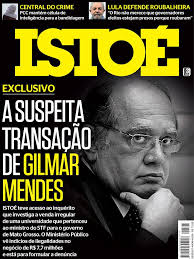
\includegraphics[height=2cm]{figuras/revista.png}
    \label{fig03a}
  }
  \quad %espaco separador
  \subfloat[Jornais]{
    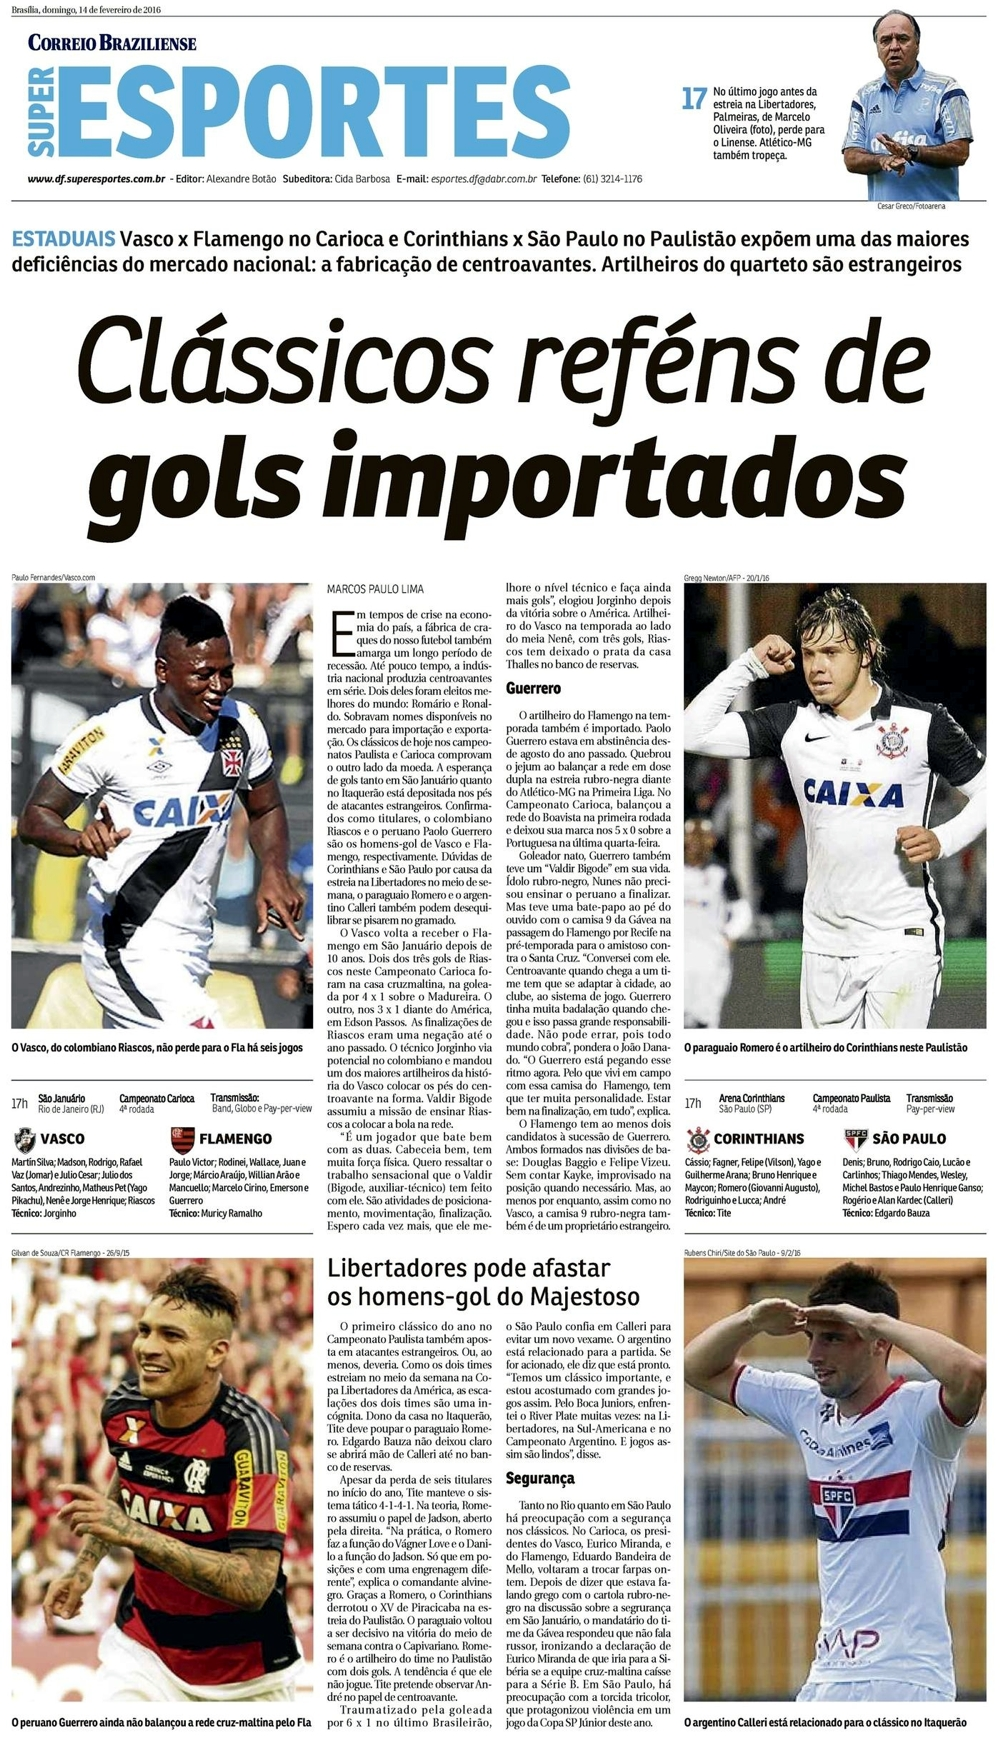
\includegraphics[height=3cm]{figuras/jornal.png}
    \label{fig3b}
  }
  \quad %espaco separador
  \subfloat[Outdors]{
    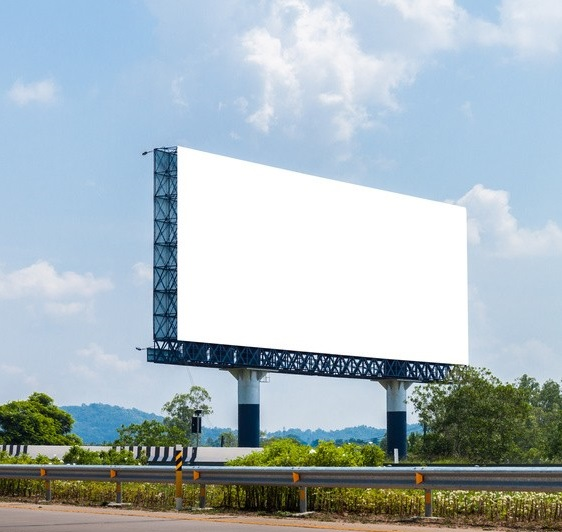
\includegraphics[height=2cm]{figuras/outdor.png}
    \label{fig3b}
  }
  \quad %espaco separador
  \subfloat[Televisões]{
    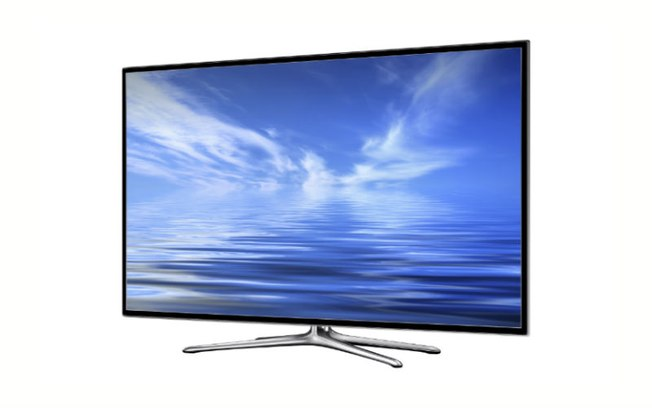
\includegraphics[height=2cm]{figuras/televisao.png}
    \label{fig3b}
  }
\label{fig1}
\end{figure}
\end{frame}

\subsection{Marketing Digital}
\begin{frame}{Marketing Digital}
\begin{center}
Publicidade tem tudo a ver com influenciar pessoas e para isso propagandas e tecnologias vem se convergindo cada vez mais para se criar um panorama de marketing.
\end{center}
\end{frame}

\begin{frame}{Marketing Digital}
\begin{figure}[h]
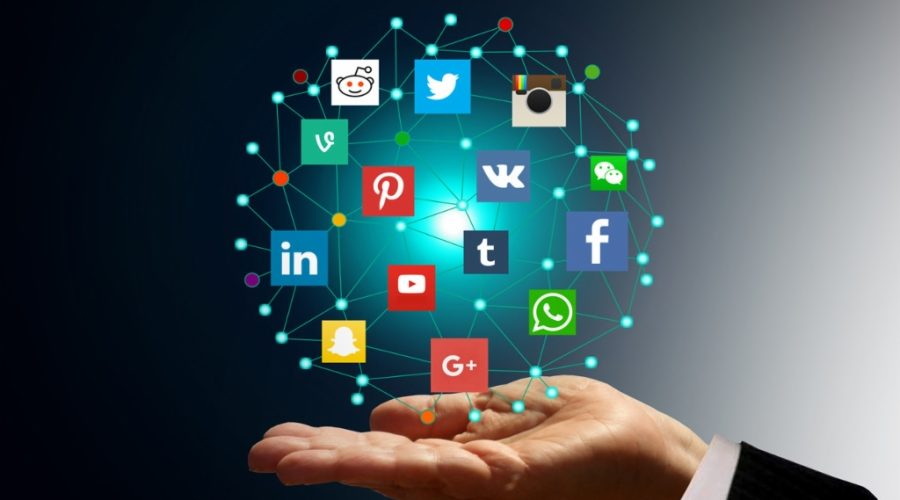
\includegraphics[width=8cm]{figuras/marketingdigital.png}
\caption{Marketing Digital}
\label{fig:siteifb}
\end{figure}
\end{frame}

\subsection{Sinalização Digital}
\begin{frame}{Sinalização Digital}
\begin{center}
Sinalização digital pode ser usada como alternativa aos outdoors, que poluem visualmente grandes cidades.
\end{center}
\end{frame}

\begin{frame}{Sinalização Digital}
\begin{figure}[h]
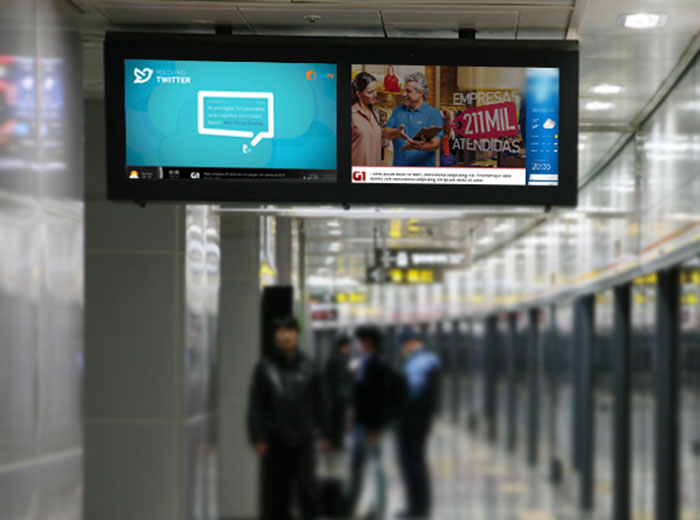
\includegraphics[width=8cm]{figuras/sinalizacaodigital.png}
\caption{Sinalização Digital}
\label{fig:siteifb}
\end{figure}
\end{frame}

\subsection{Definição do problema}
\begin{frame}{Atuais meios online}
\begin{figure}[h]
  \centering
  \subfloat[Página WEB]{
    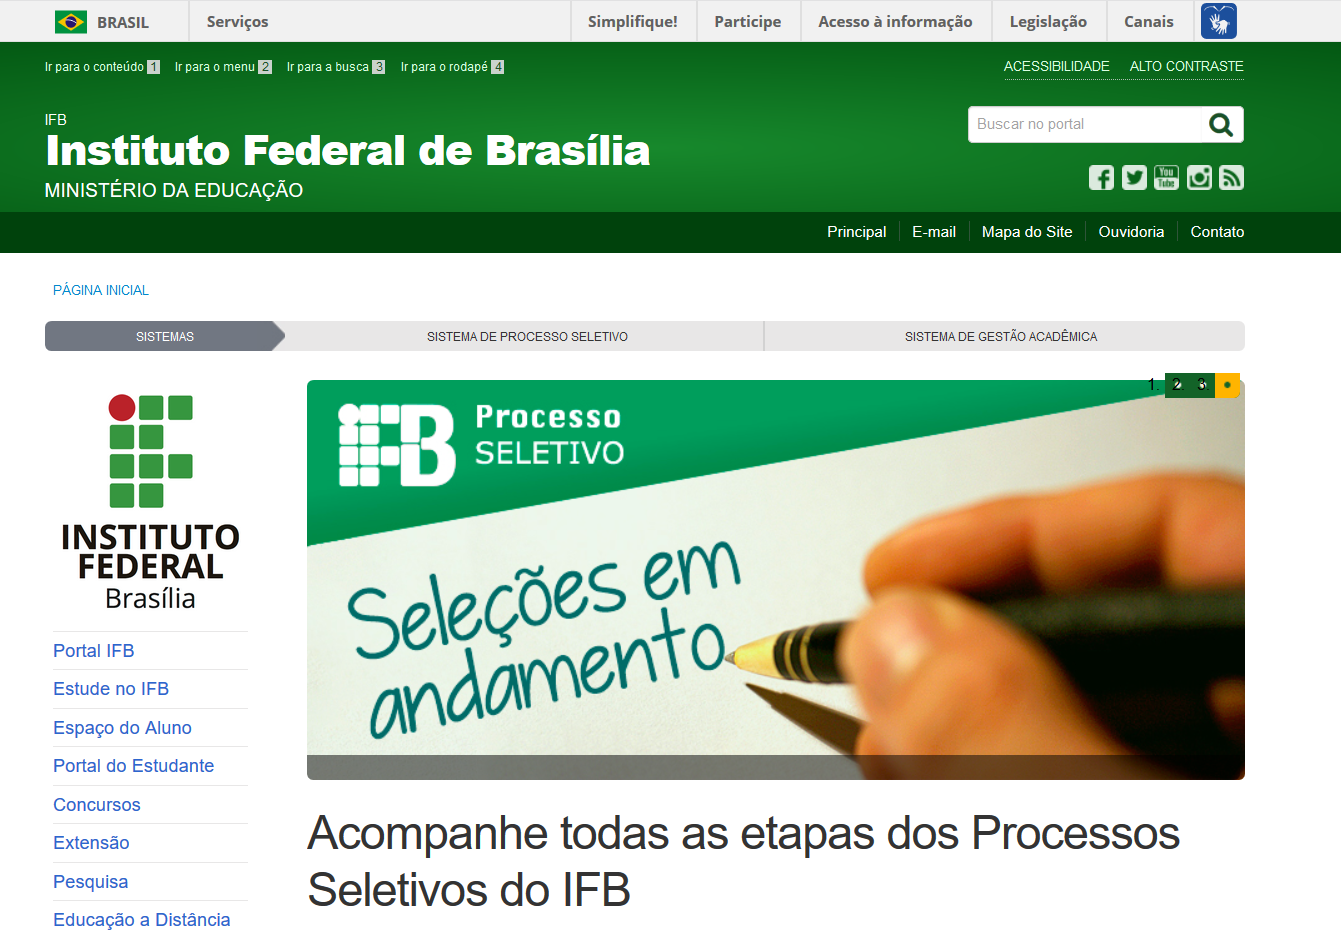
\includegraphics[height=3.5cm]{figuras/siteifb.png}
    \label{fig03a}
  }
  \quad %espaco separador
  \subfloat[Página Facebook]{
    
\includegraphics[height=3.5cm]{figuras/facebookifb.png}
    \label{fig3b}
  }
\label{fig1}
\end{figure}
\end{frame}

\begin{frame}{Atuais meios fisicamente}
\begin{figure}[h]
  \centering
  \subfloat[Panfletos]{
    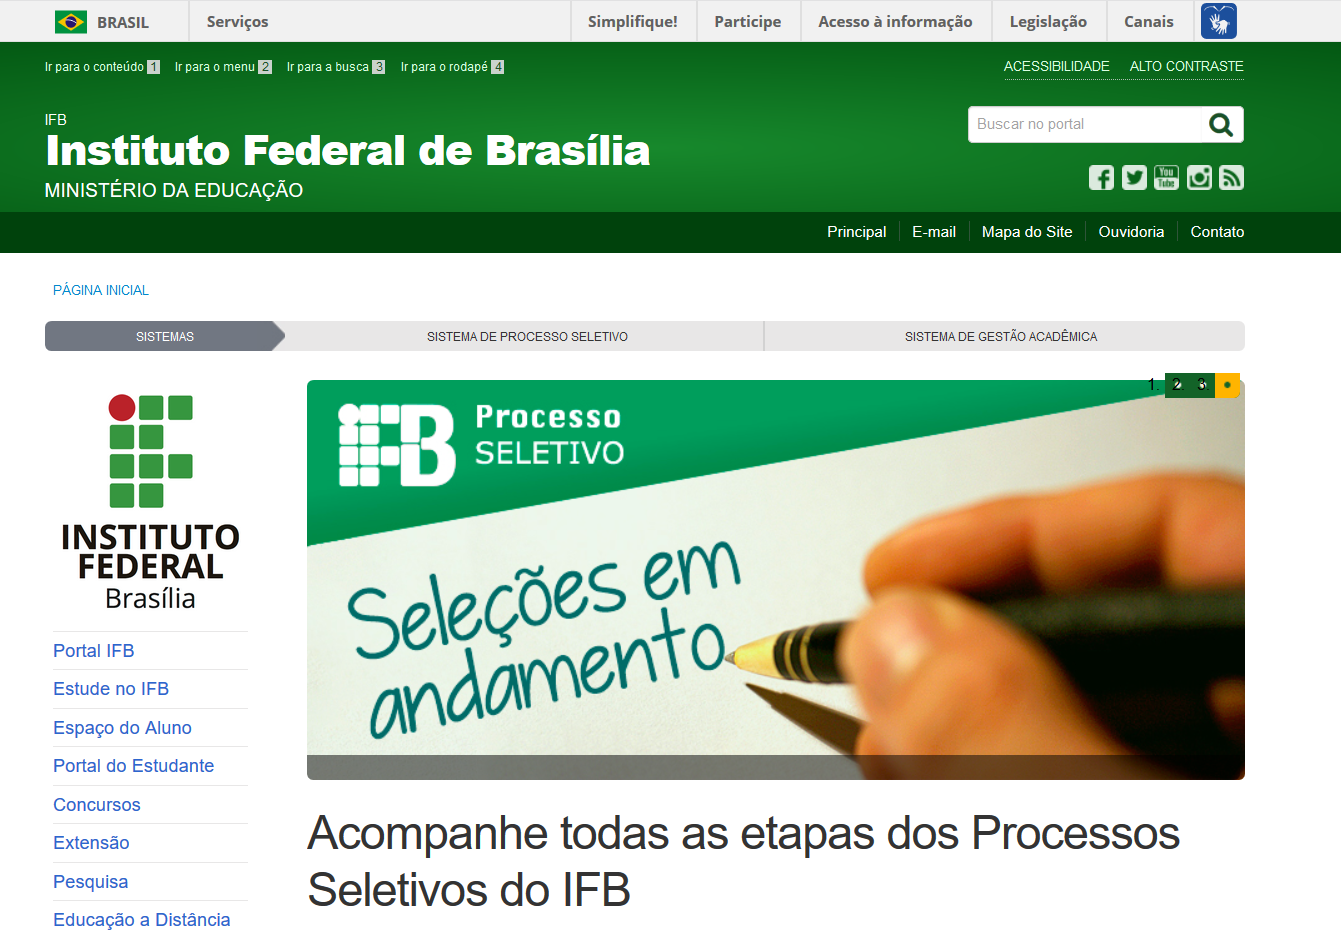
\includegraphics[height=3.5cm]{figuras/siteifb.png}
    \label{fig03a}
  }
  \quad %espaco separador
  \subfloat[Painéis]{
    
\includegraphics[height=3.5cm]{figuras/facebookifb.png}
    \label{fig3b}
  }
\label{fig1}
\end{figure}
\end{frame}

\begin{frame}{Quais são os problemas?}
\begin{itemize}
   \item Falta de integração entre os veículos de comunicação;
   \vspace{10px}
   \item Falta de interatividade com as notícias;
   \vspace{10px}
   \item Má disseminação da notícia;
   \vspace{10px}
   \item Difícil acesso;
\end{itemize}	 
\end{frame}

\subsection{Motivação e proposta}
\begin{frame}
MOTIVAÇÃO
\end{frame}

\begin{frame}
\begin{itemize}
   \item Necessidade do administrador acessar cada página e realizar uma postagem independente em cada uma delas;
   \vspace{10px}
   \item Unir os conceitos de marketing digital e sinalização digital;
   \vspace{10px}
   \item Integrar os sistemas utilizados atualmente;
   \vspace{10px}
   \item Facilitar a criação, edição e exibição de notícias;
   \vspace{10px}
   \item Desenvolver um protótipo de aplicativo mobile;
\end{itemize}

\end{frame}

\begin{frame}{Quais são as propostas?}
\begin{itemize}
   \item Usar o SIDv2 como base para implementação da versão 3;
   \vspace{10px}
   \item Unir os conceitos de marketing digital e sinalização digital;
   \vspace{10px}
   \item Integrar os sistemas utilizados atualmente;
   \vspace{10px}
   \item Facilitar a criação, edição e exibição de notícias;
   \vspace{10px}
   \item Desenvolver um protótipo de aplicativo mobile;
\end{itemize}
\end{frame}

\begin{frame}{Quais são as propostas?}
\begin{itemize}
   \item Melhorar a interatividade;
   \vspace{10px}
   \item Integrar os atuais sistemas de divulgação;
   \vspace{10px}
   \item Melhorar a forma de comunicação entre professor e aluno;
   \vspace{10px}
   \item Apresentar uma forma de implantação;
\end{itemize}
\end{frame}

\begin{frame}{Quais são as propostas?}
Melhorar a forma com que as notícias são expostas:
\begin{figure}[h]
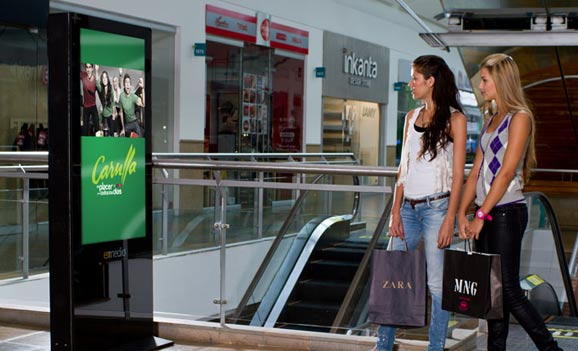
\includegraphics[width=8cm]{figuras/sinalizacao.png}
\caption{Sinalização Digital}
\label{fig:siteifb}
\end{figure}
\end{frame}

\subsection{Objetivos}
\begin{frame}{Portanto, os objetivos são...}

\end{frame}

\subsection{Metodologia}
\begin{frame}{Para isso foi necessário...}
\begin{itemize}
   \item Realizar uma revisão da bibliografia;
   \vspace{10px	}
   \item Avaliar os pontos negativos baseando-se nas necessidades do Campus;
   \vspace{10px	}
   \item Estudar a documentação da Graph API e suas ferramentas;
   \vspace{10px}
   \item Realizar as modificações que forem necessárias e não implementadas na segunda versão do SID.
   \vspace{10px}
   \item Melhorar a forma de comunicação entre professor e aluno;
   \vspace{10px}
   \item Apresentar uma forma de implantação;
\end{itemize}
\end{frame}

\section{Graph API}
\begin{frame}
Graph API
\end{frame}

\begin{frame}{Graph API}
\begin{center}
Integrar o Facebook a outros aplicativos externos. Com o uso dela é possível realizar as requisições de dados para a rede social.
\end{center}
\end{frame}

\begin{frame}{Estrutura}
\begin{figure}[h]
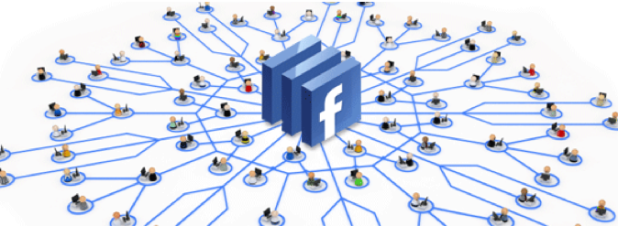
\includegraphics[width=10cm]{figuras/facebookgraph.png}
\caption{Graph Api}
\label{fig:facebookgraph}
\end{figure}
\end{frame}

\begin{frame}{Requisição de dados}
\begin{center}
Usa dos conceitos de grafo para realizar as buscas!\\
\end{center}
Com ele é possível obter dados de usuário ou de página que podem ser por exemplo: 
\begin{itemize}
   \item Postagens;
   \item Comentários;
   \item Álbuns;
   \item Fotos;
   \item Eventos;
   \item Vídeos;
\end{itemize}
\end{frame}

\begin{frame}{Detalhes}
\begin{itemize}
   \item Necessário um Token;
   \item Autenticação em conformidade com protocolo OAuth 2.0;
   \item Acesso de acordo com as permissões concedidas;
\end{itemize}
\end{frame}

\begin{frame}{Tipos de requisição}
\begin{figure}[h]
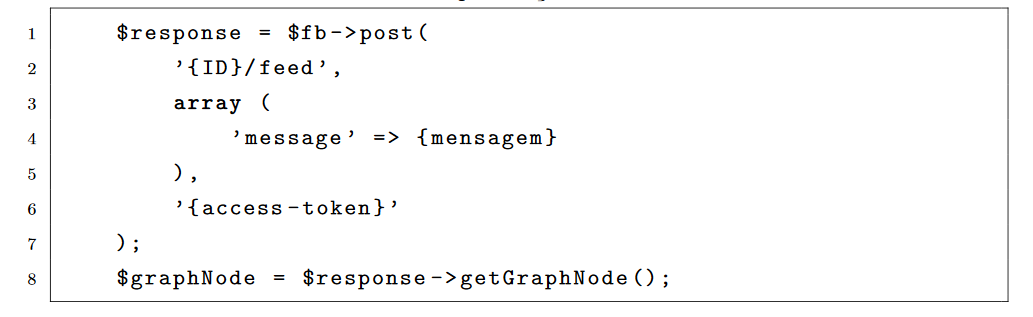
\includegraphics[width=10cm]{figuras/requisicaopost.png}
\label{fig:facebookgraph}
\end{figure}
\begin{figure}[h]
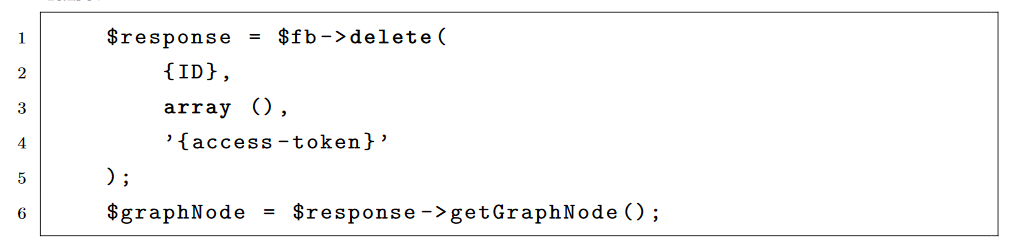
\includegraphics[width=10cm]{figuras/requisicaodelete.png}
\label{fig:facebookgraph}
\end{figure}
\end{frame}

\begin{frame}{Formas de Requisições}
\begin{figure}[h]
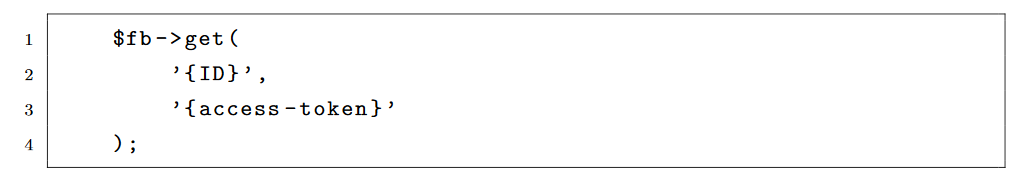
\includegraphics[width=10cm]{figuras/requisicaovertice.png}
\label{fig:facebookgraph}
\end{figure}

\begin{figure}[h]
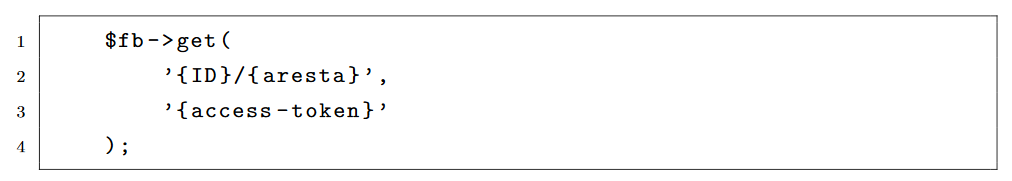
\includegraphics[width=10cm]{figuras/requisicaoaresta.png}
\label{fig:facebookgraph}
\end{figure}

\begin{figure}[h]
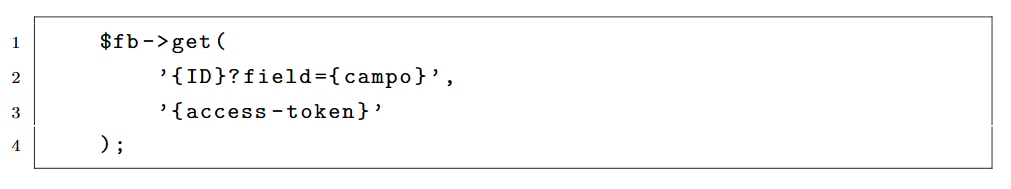
\includegraphics[width=10cm]{figuras/requisicaocampo.png}
\label{fig:facebookgraph}
\end{figure}
\end{frame}

\section{SID}
\begin{frame}
SID
\end{frame}
\subsection{Modulos}
\begin{frame}{Administrador}
Situado no servidor, é responsável por conceder ao usuário administrador as funcionalidades de gerenciamento do sistema, tais como:
\begin{itemize}
   \item Inserção;
   \item Listagem;
   \item Detalhamento;
   \item Exclusão;
   \item Edição;
\end{itemize}
\end{frame}

\begin{frame}{Submódulo API}
Situado no servidor, é responsável por:
\begin{itemize}
   \item Recuperar os dados das publicações realizadas pelo administrador no Facebook e trata-los para envio de forma formatada para os clientes. 
   \item Simular parte das funcionalidades de um Sistema de Gestão Acadêmcica, para que seja possível o consumo dos dados por um aplicativo externo, via API.
\end{itemize}
\end{frame}

\begin{frame}{Módulo Cliente}
Podendo ser situado no servidor ou em um dispositivo externo, ele é responsável por:
\begin{itemize}
   \item Realizar requisições ao submódulo API para obter os dados;
   \item Exibir de forma simples e dinâmica os dados recebidos;
   \item Realizar a troca do conteúdo que está sendo exibido de acordo com o tempo definido;
   \item Oferecer acesso a publicação completa via QRCode;
\end{itemize}
\end{frame}

\begin{frame}{Mobile}
\begin{itemize}
   \item Realizar requisições ao submódulo API para obter os dados;
\end{itemize}
\end{frame}

\subsection{Funcionalidades}
\subsubsection{Administrador}
\begin{frame}{Funcionalidades Administrador - Login}
\begin{figure}[h]
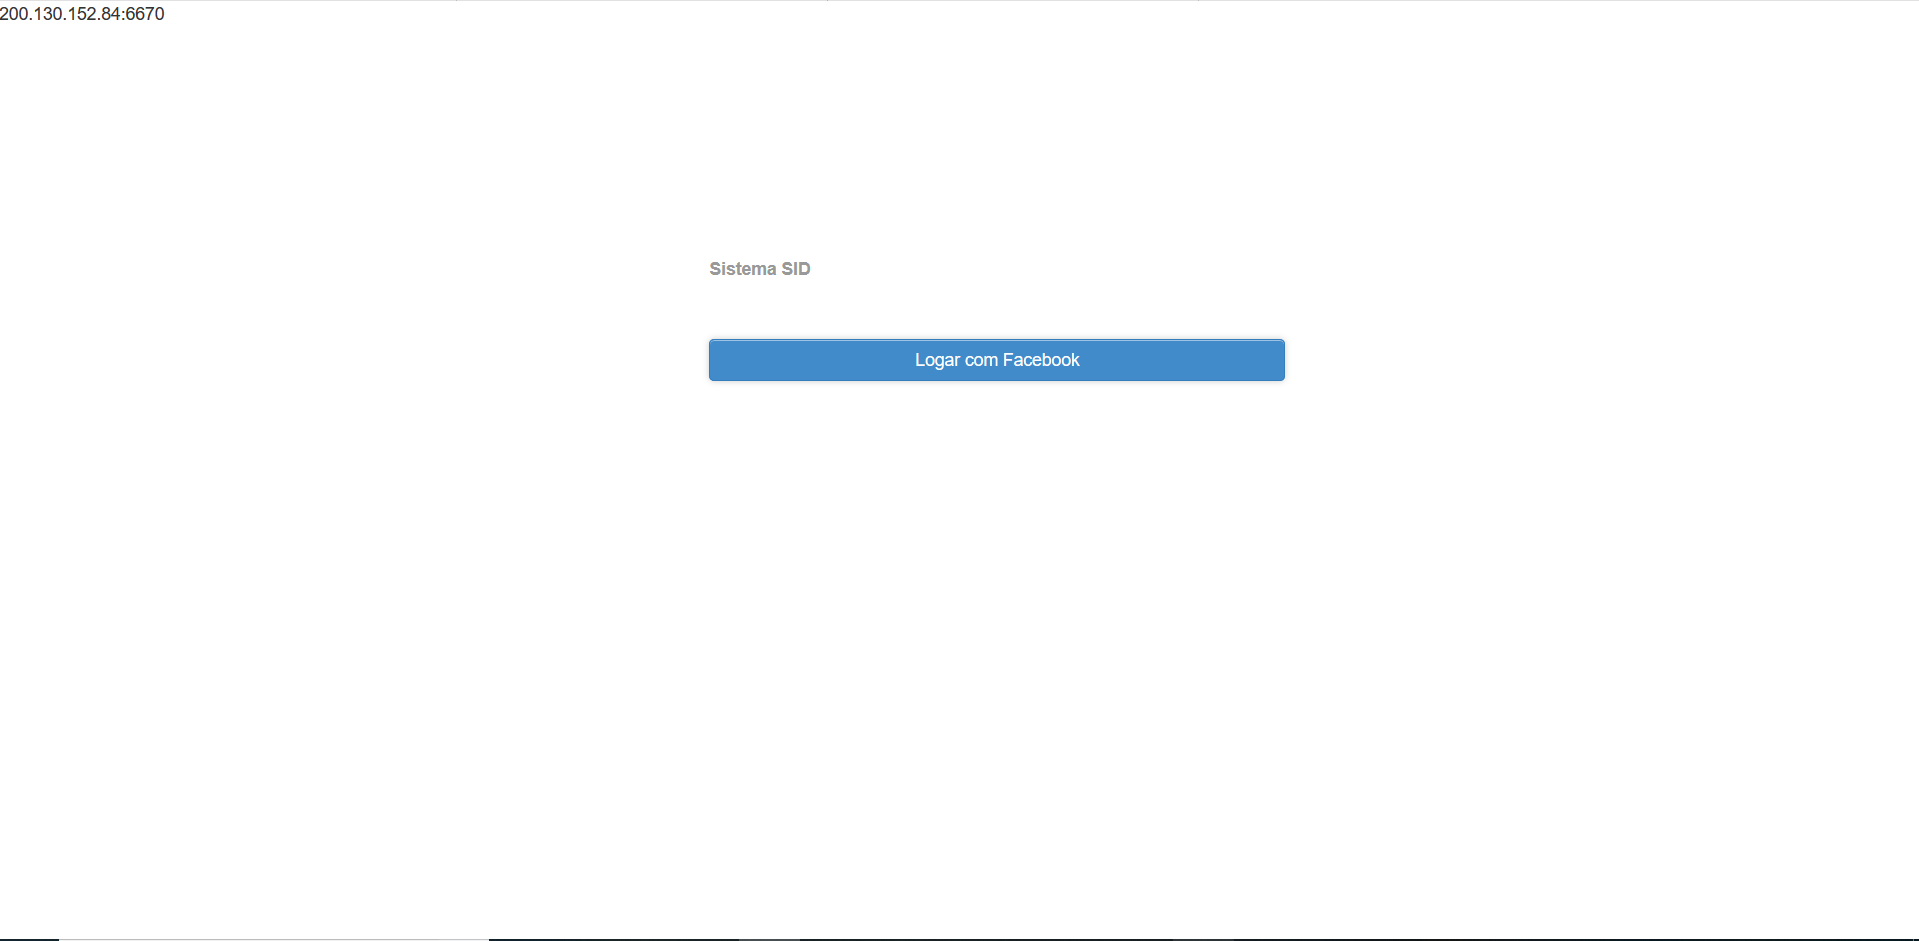
\includegraphics[width=10cm]{figuras/funcionalidadelogin.png}
\label{fig:facebookgraph}
\end{figure}
\end{frame}

\begin{frame}{Funcionalidades Administrador - Inserção}
\begin{figure}[h]
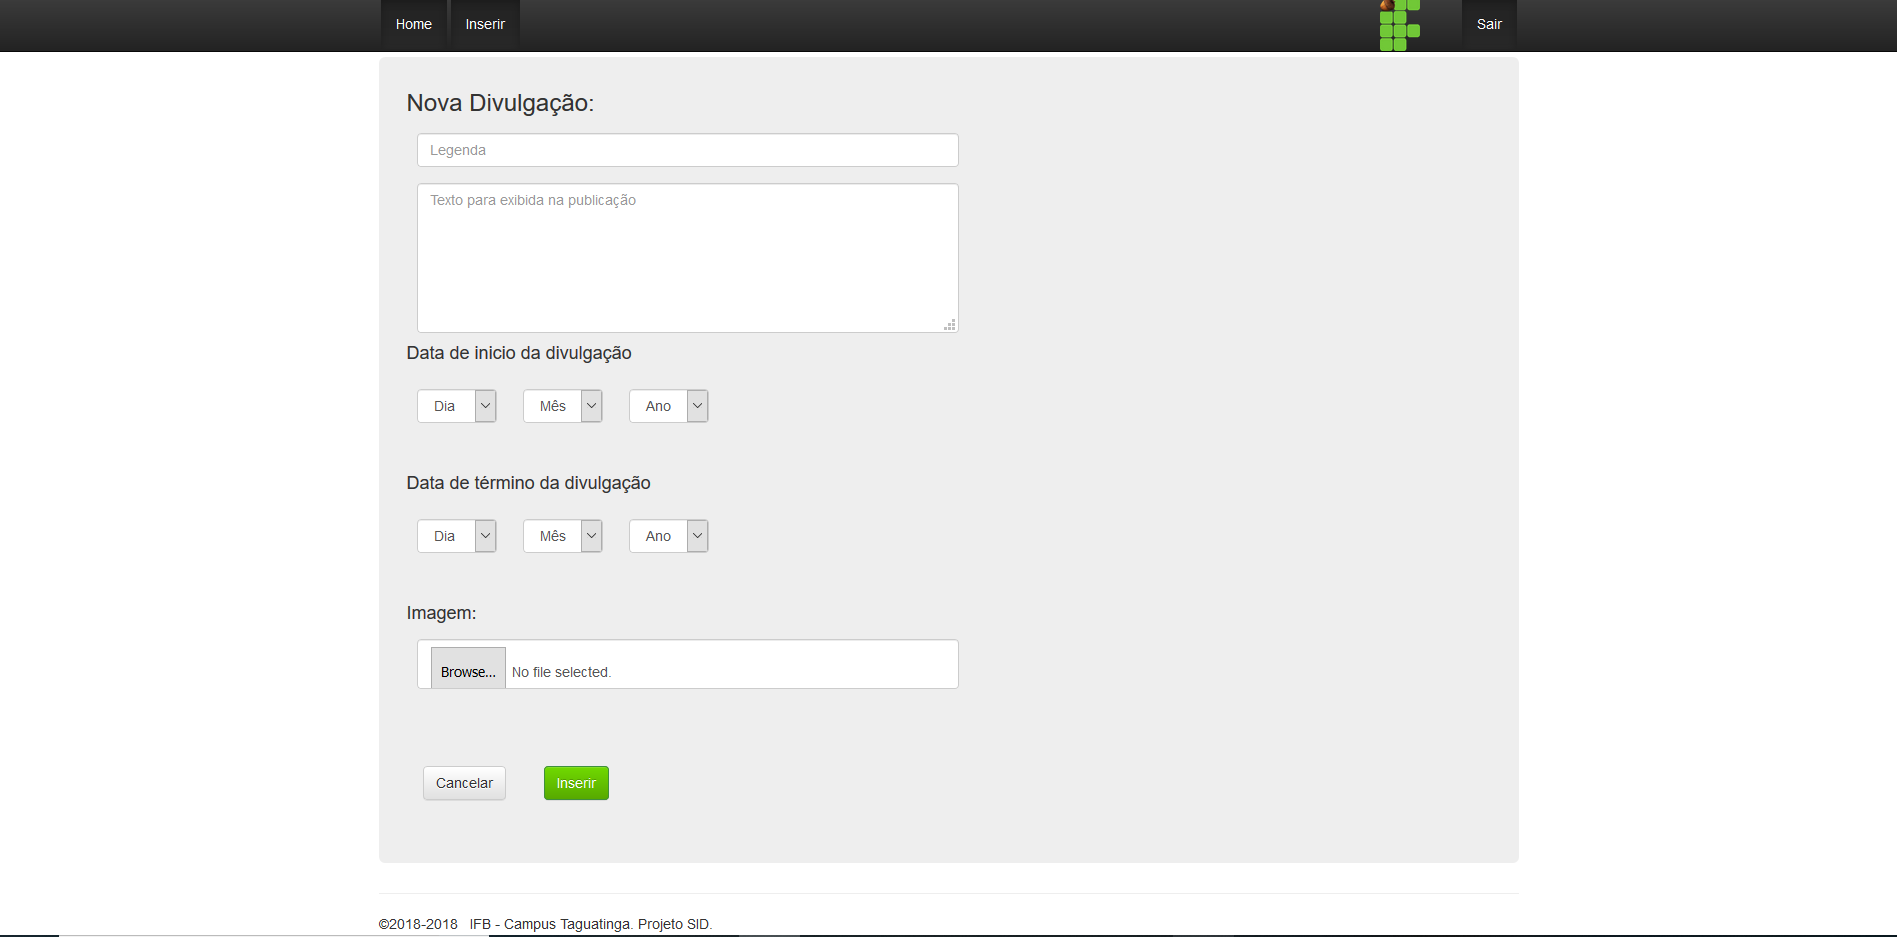
\includegraphics[width=10cm]{figuras/funcionalidadeinserir.png}
\label{fig:facebookgraph}
\end{figure}
\end{frame}

\begin{frame}{Funcionalidades Administrador - Listagem e Detalhamento}
\begin{figure}[h]
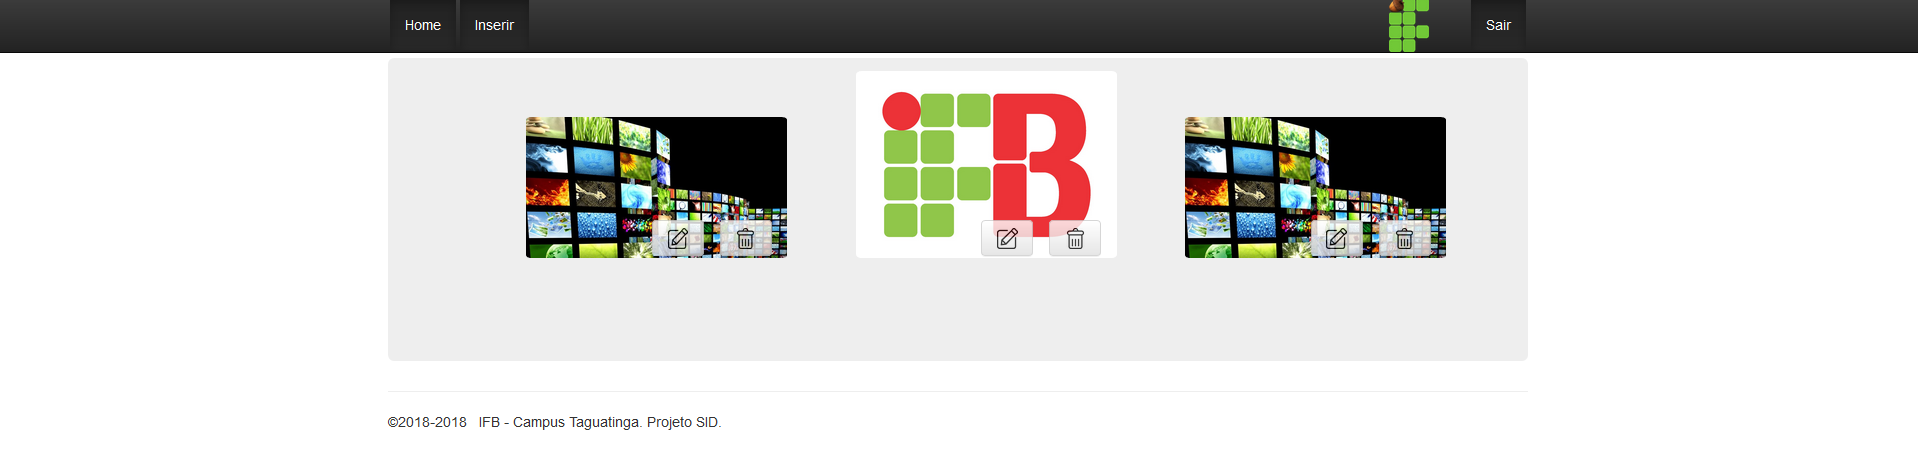
\includegraphics[width=10cm]{figuras/funcionalidadelistar.png}
\label{fig:facebookgraph}
\end{figure}
\begin{figure}[h]
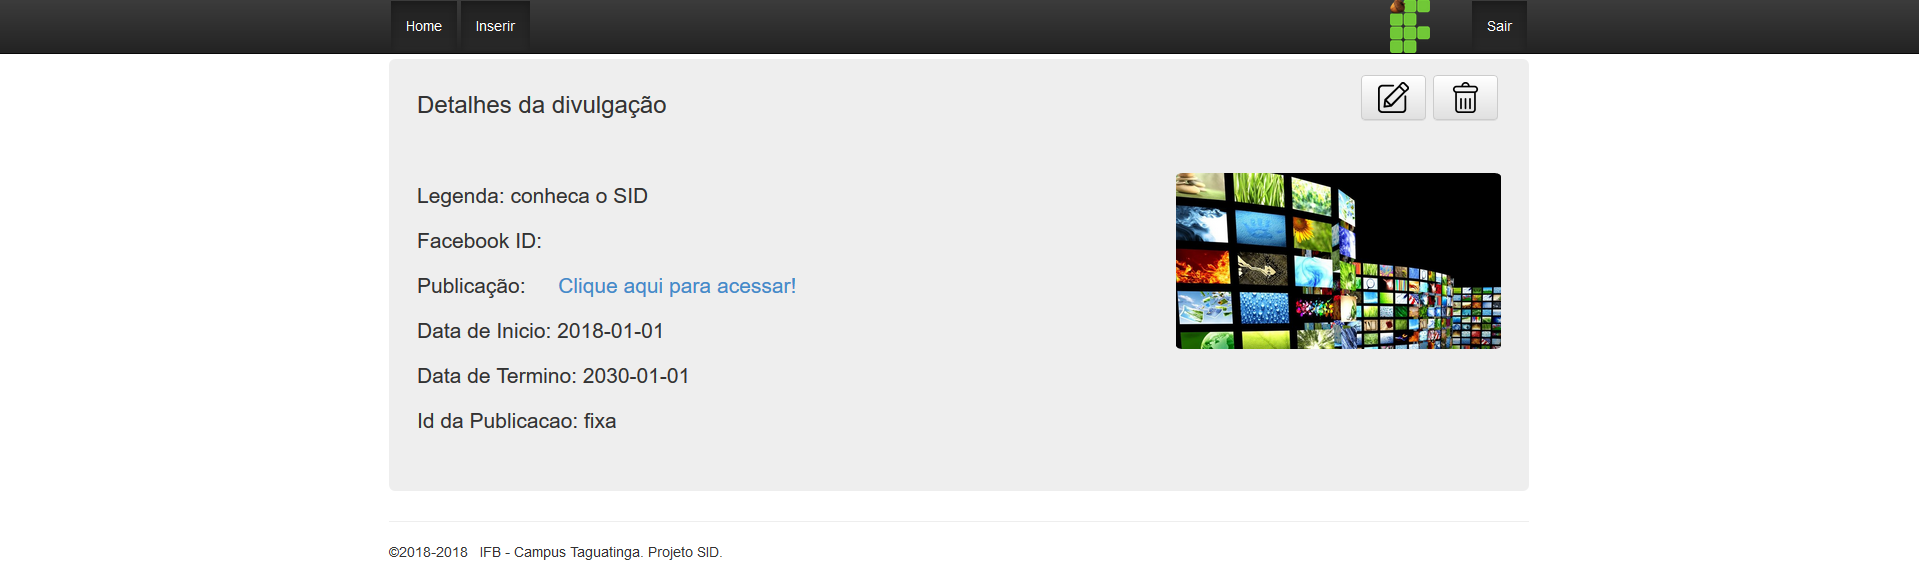
\includegraphics[width=10cm]{figuras/funcionalidadedetalhar.png}
\label{fig:facebookgraph}
\end{figure}
\end{frame}

\begin{frame}{Funcionalidades Administrador - Edição e Exclusão}
\begin{figure}[h]
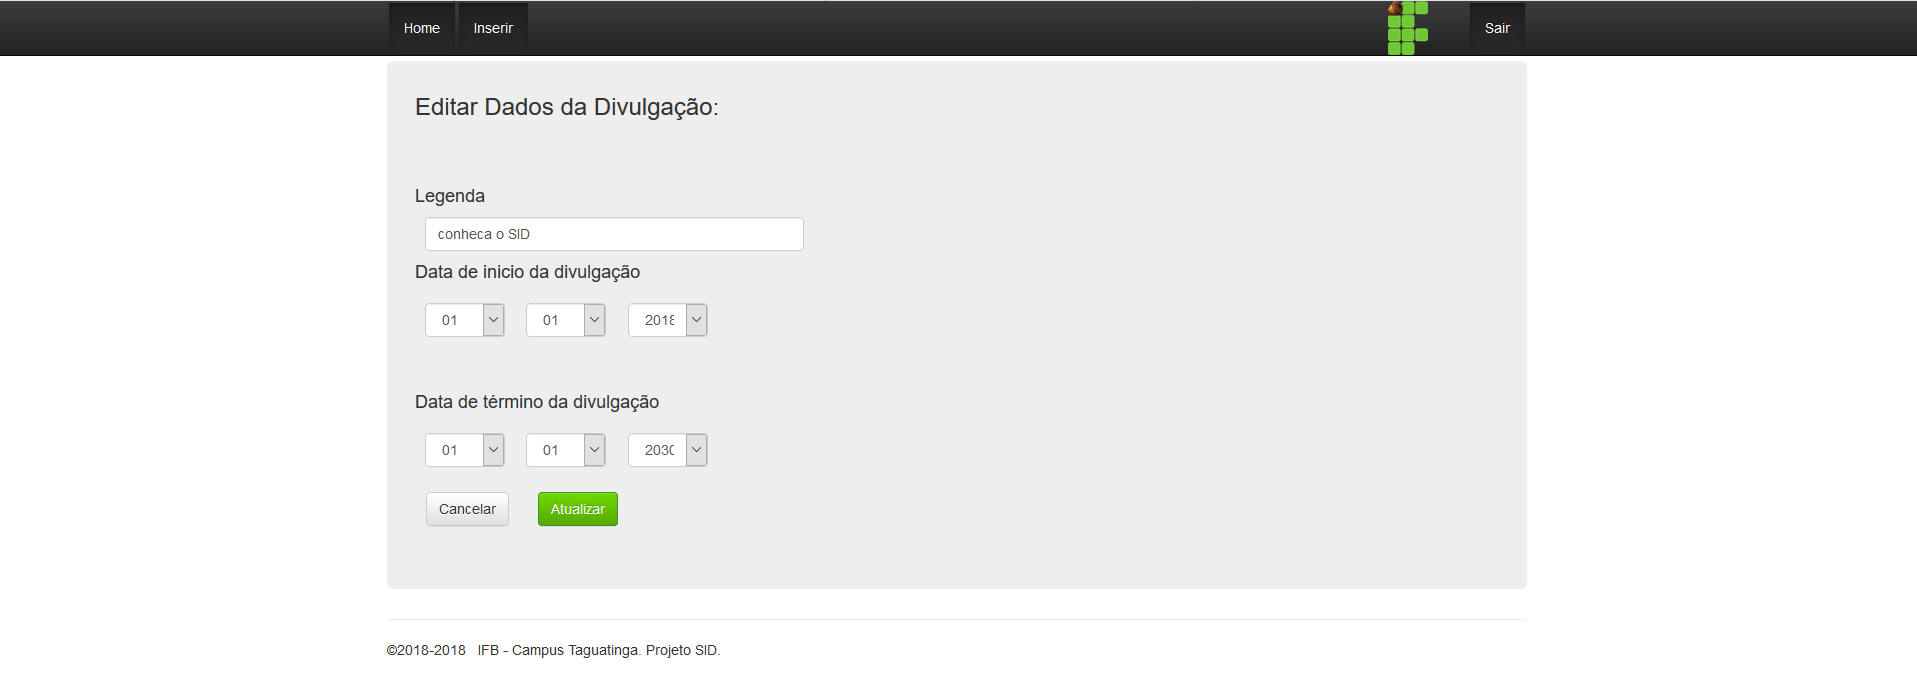
\includegraphics[width=10cm]{figuras/funcionalidadeeditar.png}
\label{fig:facebookgraph}
\end{figure}

\begin{figure}[h]

\includegraphics[width=10cm]{figuras/funcionalidadedeletar.png}
\label{fig:facebookgraph}
\end{figure}
\end{frame}

\subsubsection{Administrador}
\begin{frame}{Funcionalidades Cliente - exibição}
\begin{figure}[h]
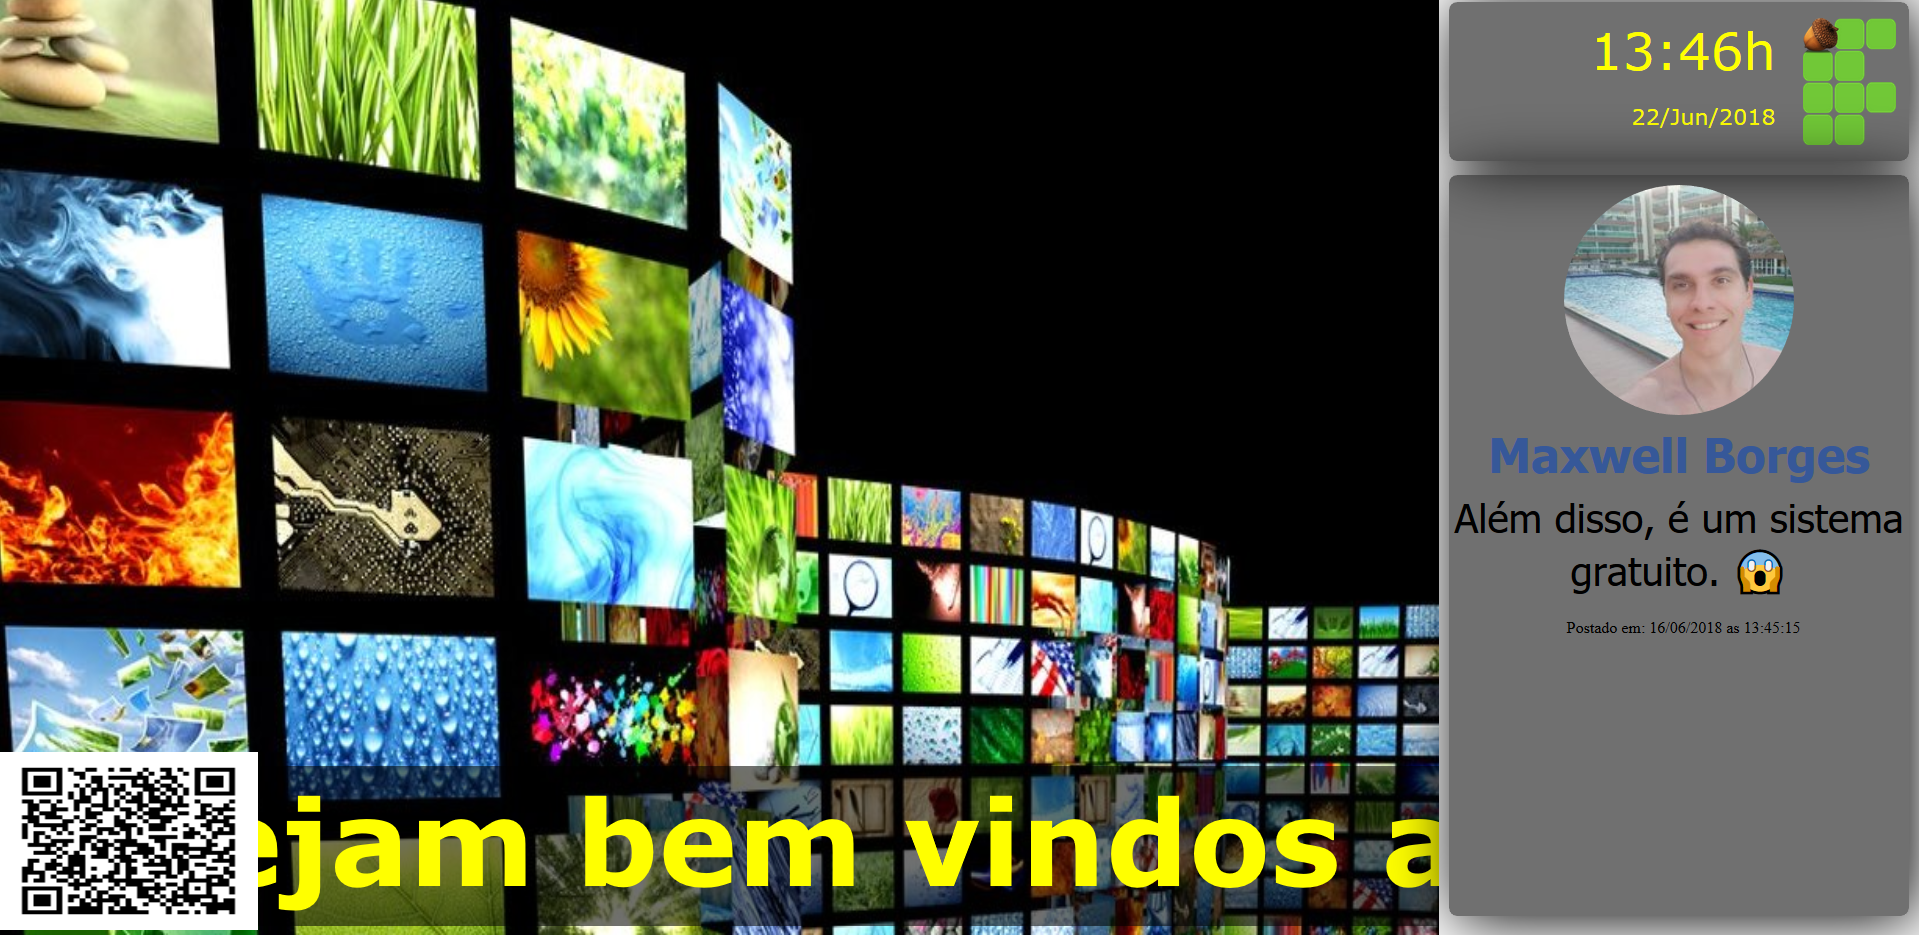
\includegraphics[width=10cm]{figuras/funcionalidadeexibir.png}
\label{fig:facebookgraph}
\end{figure}
\end{frame}

\subsubsection{Mobile}
\begin{frame}{Funcionalidades Mobile - exibição}
\begin{figure}[h]
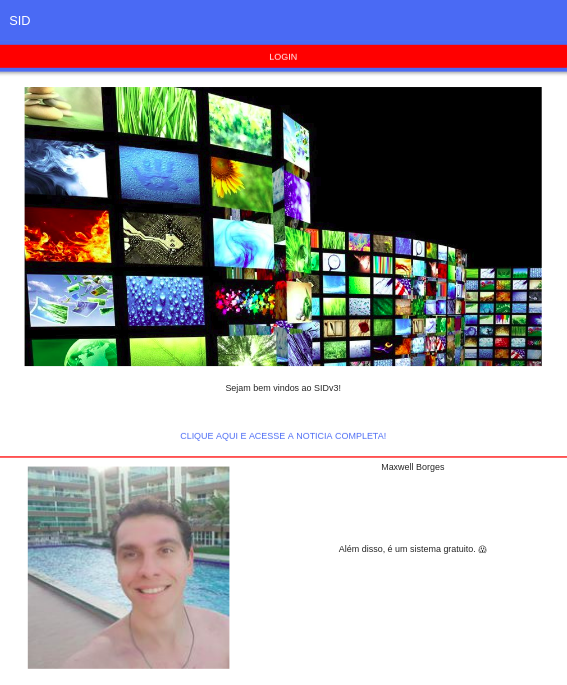
\includegraphics[width=5cm]{figuras/mobile1.png}
\label{fig:facebookgraph}
\end{figure}
\end{frame}

\begin{frame}{Funcionalidades Mobile - Login}

\end{frame}


\begin{frame}{Funcionalidades Mobile - Professor}
\begin{figure}[h]
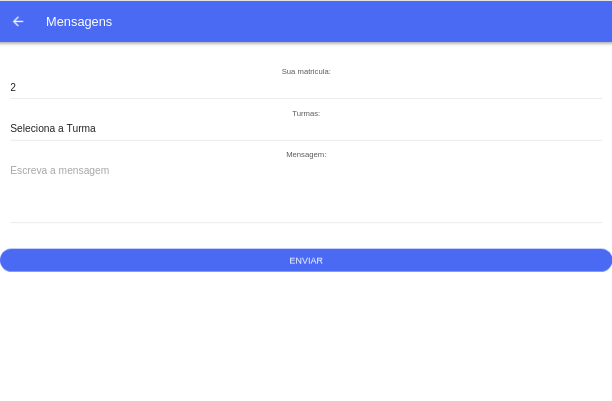
\includegraphics[width=6cm]{figuras/mobile2.png}
\label{fig:facebookgraph}
\end{figure}
\end{frame}

\begin{frame}{Funcionalidades Mobile - Aluno}
\begin{figure}[h]
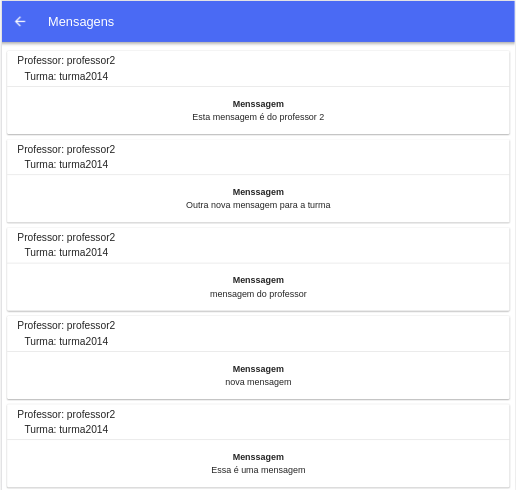
\includegraphics[width=6cm]{figuras/mobile3.png}
\label{fig:facebookgraph}
\end{figure}
\end{frame}

\section{Resultados}
\begin{frame}
RESULTADOS
\end{frame}

\begin{frame}{Resultados}
Resultados - Comparação com os demais
\end{frame}

\section{Conclusão e trabalhos futuros}
\begin{frame}

\end{frame}

\section{Final}
\begin{frame}
FIM
\end{frame}

\end{document}